
%(BEGIN_QUESTION)
% Copyright 2011, Tony R. Kuphaldt, released under the Creative Commons Attribution License (v 1.0)
% This means you may do almost anything with this work of mine, so long as you give me proper credit

This furnace temperature control system does not work as well as operations personnel would like.  The temperature drifts around, unable to hold steady at setpoint, despite many attempts to adjust the ``tuning'' parameters in the TIC (proportional, integral, and derivative):

$$\includegraphics[width=15.5cm]{i00714x01.eps}$$

Finally a fellow instrument technician happens to notice the pressure gauge (PG) at the fuel oil pump discharge indicate an unsteady pressure.  Rather than hold constant at some value, the fuel oil pressure seems to rise and fall seemingly at random.

\vskip 10pt

Design a solution for this temperature-stability problem using a {\it cascade} control strategy, explaining the reasoning behind your solution.

\vskip 20pt \vbox{\hrule \hbox{\strut \vrule{} {\bf Suggestions for Socratic discussion} \vrule} \hrule}

\begin{itemize}
\item{} Can you think of any solutions to this control dilemma other than cascade?
\item{} Why do you suppose there is a return valve in the fuel oil plumbing?
\item{} Explain what will happen in this system if someone suddenly shuts off the return valve, from its normal position.
\item{} Explain what will happen in this system if someone suddenly opens up the return valve, from its normal position.
\end{itemize}

\underbar{file i00714}
%(END_QUESTION)





%(BEGIN_ANSWER)

There are multiple solutions one could implement to fix this problem.  Here is one:

$$\includegraphics[width=15.5cm]{i00714x02.eps}$$

%(END_ANSWER)





%(BEGIN_NOTES)

Here is a solution that does not rely on cascade or any other control strategy per se:

$$\includegraphics[width=15.5cm]{i00714x03.eps}$$

%INDEX% Control, strategies: cascade
%INDEX% Process: combustion furnace 

%(END_NOTES)


